\section{Grundlagen}\label{sec:grundlagen}

In der Informatik nimmt das Optimieren von Programmcode eine wichtige Aufgabe ein.
Indem überflüssige Schleifendurchläufe eingespart oder unerreichbarer Code eliminiert wird,
kann das Programm Zeit und Ressourcen einsparen. 
Während manche Optimierungen vom Programmierer vorgenommen werden können, sind andere nur 
durch den Compiler möglich.
Der Compiler enthält zum Beispiel einen maschinenunabhängigen Codeoptimierer, der global Optimierungen
im Programm vornehmen kann, indem er verschiedenen Techniken wie die Datenflussanalyse anwendet~\cite{ullman2008}.

\noindent Eine weitere Möglichkeit für Optimierungen ist die Verwendung von \textit{E-Graphs} und \textit{Equality Saturation}.
Hierbei werden vor allem mathematische Ausdrücke in effizientere umgewandelt.
Um diesen Prozess zu verstehen, startet dieses Kapitel zuerst mit einem naiven Ansatz und zeigt anhanddessen Probleme auf, die
während der Optimierung auftreten können.

\subsection{Naives Optimieren}

Gegeben sei ein mathematischer Ausdruck, zum Beispiel: $a * 1$. Um diesen Ausdruck umzuformen, kann eine \textit{rewrite rule} eingesetzt werden.
Eine \textit{rewrite rule} beschreibt die Umformung eines Ausdrucks in einen anderen. Als Beispiel sei hier folgende Regel gegeben: $x * 1 \Leftrightarrow x \;\; (1)$.
Angewendet auf den obigen Ausdruck würde sich folgendes ergeben: $a * 1  \overset{(1)}{\Leftrightarrow} a$.
Die Anwendung dieser \textit{rewrite rule} ist nur möglich, weil die Regel \textit{matcht}. Das bedeutet, dass der Ausdruck und die linke Seite der Regel identisch sind 
(abgesehen vom Namen der Variablen). Die folgende \textit{rewrite rule} würde nicht \textit{matchen} und damit auch nicht angewendet werden können: $\frac{x}{x} \Leftrightarrow 1$.
Mit diesen Bausteinen lässt sich bereits ein naiver Algorithmus anfertigen, der in Abbildung~\ref{alg:ausdruck1} dargestellt ist.

\begin{algorithm}[H]
  \caption{Naiver Algorithmus zur Optimierung von Ausdrücken}\label{alg:ausdruck1}
  \begin{algorithmic}
    \Function{optimiere\_Ausdruck}{ausdruck}
    \State $rules \gets [\ldots]$
    
    \While{$ausdruck\_alt \neq ausdruck$}
      \State $ausdruck\_alt \gets ausdruck$

      \For{rule in rules}
        \If{match(ausdruck, rule)}
        \State apply(ausdruck, rule)
        \EndIf
      \EndFor
    \EndWhile

    \State \Return ausdruck
    \EndFunction
  \end{algorithmic}
\end{algorithm}

Dieser Algorithmus wendet solange \textit{rewrite rules} auf einen Ausdruck an, bis keine Veränderung mehr auftritt.
Zwar zeichnet sich diese Lösung durch ihre Einfachheit aus, kommt aber auch mit Nachteilen.
So läuft er bereits bei einfachen Beispielen in lokale Optima. 
Als Beispiel dient hier der Ausdruck $(a * 2) / 2$, der mit den Regeln $(x * y) / z \Leftrightarrow x * (y / z), x / x \Leftrightarrow 1, x * 1 \Leftrightarrow x$ 
zum Ausdruck $a$ umgeformt werden kann.
Wird stattdessen eine weitere Regel eingefügt, zum Beispiel $x * 2 \Leftrightarrow x << 1$, könnte der Algorithmus auch mit folgendem Ausdruck enden: $(a << 1) / 2$.
Das Ergebnis hängt also von der Reihenfolge der verwendeten Regeln ab. Dieses Problem ist allgemein als das \textit{Phase Ordering Problem} bekannt~\cite{phaseorder-2009}.
Ein weiteres Problem sind kurzsichtige Heuristiken, die dazu tendieren, die Optimalität von Ausdrücken nicht über mehrere Schritte, sondern nur für den momentanen Schritt
zu verfolgen~\cite{phaseorder-2009}.

\noindent Um diese Probleme zu umgehen, kann der vorherige Algorithmus um eine Liste erweitert werden (siehe~\footnote{\url{https://www.cole-k.com/2023/07/24/e-graphs-primer/}}).
Diese Liste speichert alle erzeugten Ausdrücke ohne Duplikate. Nun wird versucht, alle möglichen Regeln auf die Ausdrücke in der Liste anzuwenden. 
Dies setzt der nächste Algorithmus in Abbildung~\ref{alg:ausdruck2} um.

\begin{algorithm}[H]
  \caption{Verbesserter, naiver Algorithmus zur Optimierung von Ausdrücken}\label{alg:ausdruck2}
  \begin{algorithmic}
    \Function{optimiere\_Ausdruck}{ausdruck}
    \State $rules \gets [\ldots]$
    \State $ausdruecke \gets list()$
    
    \While{$len(ausdruecke) \neq laenge\_alt$}
      \State $laenge\_alt \gets len(ausdruecke)$

      \For{ausdruck in ausdruecke}
        \For{rule in rules}
          \If{match(ausdruck, rule)}
          \State new\_ausdruck = apply(ausdruck, rule)
          \State ausdruecke.add(new\_ausdruck)
          \EndIf
        \EndFor
      \EndFor
    \EndWhile

    \State \Return ausdruecke.get\_best()
    \EndFunction
  \end{algorithmic}
\end{algorithm}

Am Ende der Ausführung steht eine komplette Liste mit allen möglichen Konfigurationen des Ursprungsausdrucks zur Verfügung, aus der man den optimalen Ausdruck extrahieren kann.
Zwar konnte hier das \textit{Phase Ordering Problem} umgangen werden, jedoch hat der Algorithmus eine exponentielle Laufzeit.
\textit{E-Graphs} sind Datenstrukturen, die diese Probleme lösen können.

\subsection{E-Graphs}

Um ein grundlegendes Verständnis von \textit{E-Graphs} zu erlangen, werden zunächst einige wichtige Konzepte vorgestellt.

\subsubsection{Äquivalenzrelation}

Eine Äquivalenzrelation beschreibt eine Gleichwertigkeit zwischen Objekten, die folgende Eigenschaften erfüllen muss~\cite{Ehrig2001}:

\begin{itemize}
  \item \textbf{Reflexivität} Das Objekt ist gleichwertig zu sich selbst.
  \item \textbf{Symmetrie} Wenn Objekt $a$ zu Objekt $b$ gleichwertig ist, gilt das auch andersherum.
  \item \textbf{Transitivität} Wenn Objekt $a$ zu Objekt $b$ gleichwertig ist, und Objekt $b$ zu Objekt $c$, dann gilt auch, dass $a$ zu $c$ gleichwertig ist.
\end{itemize}

Als Beispiel dienen hier Schuhe verschiedener Marken. Zwei Schuhe $a, b$ sind bzgl. ihrer Größe äquivalent, wenn sie dieselbe Schuhgröße haben. 

\subsubsection{Äquivalenzklasse}

Eine Äquivalenzrelation teilt eine Menge von Objekten in Äquivalenzklassen klein, in denen die Objekte jeweils die drei oben genannten Eigenschaften erfüllen~\cite{Ehrig2001}.
Die Schuhe werden also bzgl. ihrer Größe in die Äquivalenzklassen \textit{Schuhgröße} eingeteilt.

\subsubsection{Zusammenhang zu E-Graphs}

Ein E-Graph besteht aus zwei Komponenten: \textit{E-Classes} und \textit{E-Nodes}. Abbildung~\ref{fig:egraphexp} zeigt einen beispielhaften E-Graph.
\textit{E-Nodes} sind dabei weiß und \textit{E-Classes} beige eingefärbt.

\begin{figure}[H]
  \centering
  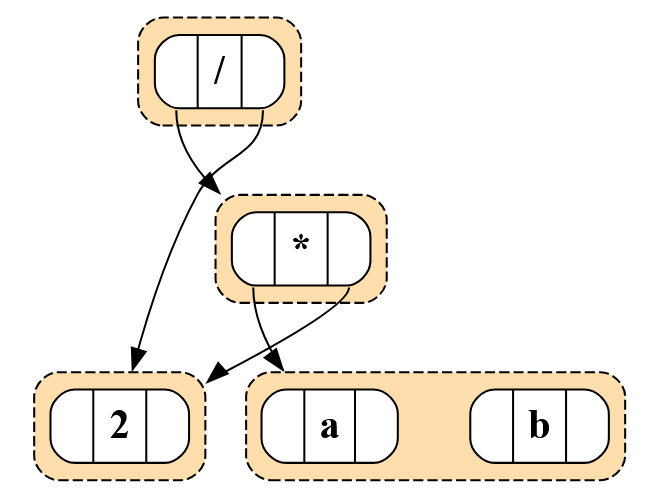
\includegraphics[scale=0.5]{../fig/egraph_exp.png}
  \caption{Beispiel eines E-Graphs, was die Ausdrücke $(a * 2) / 2$ und $(b * 2) / 2$ enthält}
  \label{fig:egraphexp}
\end{figure}

\textit{E-Classes} sind Äquivalenzklassen mit \textit{E-Nodes}, die äquivalent zueinander sind. Im Beispiel~\ref{fig:egraphexp} sind $a$ und $b$ äquivalent zueinander.
Als Argumente von \textit{E-Nodes} werden \textit{E-Classes} übergeben. Im Beispiel~\ref{fig:egraphexp} wird dem \textit{E-Node} $*$ die \textit{E-Class} mit den beiden 
\textit{E-Nodes} $a$ und $b$ und die \textit{E-Class} mit dem \textit{E-Node} $2$ übergeben. Es wird also ausgenutzt, dass $a$ und $b$ in der gleichen \textit{E-Class}
sind. 

\subsubsection{Implementierung von E-Graphs}

\textit{E-Graphs} können auf unterschiedliche Weise implementiert werden. Die in dieser Arbeit benutzte stammt aus dem Paper~\cite{2021-egg}, das \textit{egg} vorstellt 
(siehe verwandte Arbeiten~\ref{sub:verwandtearbeiten}). Ein \textbf{E-Graph} wird damit als Tuple $(\mathbf{U}, \mathbf{M}, \mathbf{H})$ mit folgenden Eigenschaften definiert:

\begin{itemize}
  \item $\mathbf{U}$ Eine Union-Find-Datenstruktur, die eine Äquivalenzrelation über IDs abspeichert.
  \item $\mathbf{M}$ Eine (Hash)-map, die IDs von E-Classes auf E-Classes abbildet. 
  \item $\mathbf{H}$ Eine (Hashcons)-map, die E-Nodes auf IDs von E-Classes abbildet.
\end{itemize}

Der \textit{E-Graph} als Datenstruktur für Beispiel~\ref{fig:egraphexp} würde also wie folgt aussehen.

\begin{itemize}
  \item $\mathbf{U}$: \{ID1\}, \{ID2\}, \{ID3\}, \{ID4, ID5\} 
  \item $\mathbf{M}$: $ID1 \rightarrow EClass(\ldots)$, $ID2 \rightarrow EClass(\ldots)$, $ID3 \rightarrow EClass(\ldots)$, \ldots 
  \item $\mathbf{H}$: $/ \rightarrow ID1$, $* \rightarrow ID2$, $2 \rightarrow ID3$, $a \rightarrow ID4$, $b \rightarrow ID5$
\end{itemize}



\subsection{Equality Saturation}

\textit{Equality Saturation} beschreibt eine iterative Methode, die solange \textit{rewrite rules} auf einen E-Graph anwendet, bis sich keine Änderungen mehr ergeben. 
Der E-Graph gilt damit als \textit{saturiert}.
In der zweiten Phase kann mithilfe einer Kostenfunktion der optimale Ausdruck aus dem E-Graph extrahiert werden.
Obwohl der Extraktionsschritt NP-schwer ist, ist es in der Praxis dennoch möglich, durch Anwendung verschiedener Methoden ein optimales Ergebnis in kurzer Zeit zu erhalten
~\cite{phaseorder-2009}. 
